\chapter{Resultaten}
We hebben verschillende kernels ontwikkeld. We hebben alle kernels uitgevoerd voor verschillende waardes van $R$ en $I$ en de tijd gemeten die het duurt om de kernel uit te voeren. Deze tijd bevat niet de tijd die nodig is om het geheugen op te vullen. De tijd is gemeten met behulp van de profiling informatie die de OpenCL-API ons aanbiedt. Voor meer informatie zie hoofdstuk 4.4.1 in de handleiding van AMD \cite{amd}. De metingen zijn tot op de nano-seconde nauwkeurig. \cite[p.~4-13]{amd}

Uit de gemeten tijd kunnen we dan de rekenkracht berekenen. We doen dit door het aantal flop voor een optimale implementatie te delen door de uitvoeringstijd. We berekenen het aantal flop met de formules uit hoofdstuk \ref{h:kernels}.

\section{Invloed van R voor kernels die $f(\T, \mUUU)$ berekenen}
\label{h:invlR}
We hebben float16x16x16 laten uitvoeren $I$ gelijk aan 64, 128 en 320 en $R$ oplopend van 1 tot en met 4000. Het resultaat ziet u in figuur \ref{invlR1200}.

Het is duidelijk te zien dat de rekenkracht in het begin lineair groeit tot het bijna de maximale rekenkracht bereikt heeft. Deze lineaire groei is nog duidelijker zichtbaar in \ref{invlR100}. We kunnen deze groei als volgt verklaren. Als $R$ laag is, is de rekenverhouding ook laag. Dit betekent dat de bandbreedte het knelpunt is die de rekenkracht beperkt. Op figuur \ref{haalF} zien we dat de rekenverhouding lineair stijgt met $R$ voor eenzelfde $I$. Dit betekent dat ook de rekenkracht lineair zal stijgen zolang het kantelpunt nog niet bereikt is.

Na de groei is er een geleidelijke overgang naar een quasie constante rekenkracht. De geleidelijke overgang verklaren we als volgt. Aan het begin van de overgang zijn alle work-items constant aan het wachten tot ze aan de beurt zijn om een geheugenoperatie uit te voeren. Dit omdat de rekenverhouding veel te laag is. Naarmate $R$ groter wordt is er meer rekenwerk en zal het langer duren voor een work-item weer moet wachten voor die aan de beurt is om een geheugenoperatie uit te voeren waardoor er ook minder work-items in de 'wachtrijen' moeten wachten. Deze 'wachtrijen' worden korter en korter naarmate $R$ groter wordt tot ze op het einde van de overgang quassie niet meer bestaan.

Na de overgang blijft de rekenkracht, op een uitzondering na, quassie constant. We zitten dan aan de maximale rekenkracht. Omdat $R$ hier groot is, zal de rekenverhouding ook hoog zijn waardoor de bandbreedte het geheugen niet meer zal hinderen. 

Bij $I=320$ doet er zich een interessant fenomeen voor. Bij $R=430$ zakt de rekenkracht terug van 1570 Gflop/s naar ongeveer 1300 Gflop/s. Het is ook opvallend dat de schommelingen na de terugval groter zijn. We vermoeden dat wanneer $R$ groter wordt dan 430, de caches niet zo goed meer werken. Het is immers zo dat de traagheid van het globaal geheugen variabel is en dat de traagheid van de caches constant is. Een andere factor zijn de kanaalconflicten. Als de timing een beetje ongelukkig is kan er zich een kanaalconflict voordoen dat zich anders niet had voorgedaan.

In figuur \ref{invlR100} zien we zeer duidelijk dan voor $I = 64$ de rekenkracht stapsgewijs groeit in de groeifase. We kunnen dit niet verklaren.

\begin{figure}
\centering
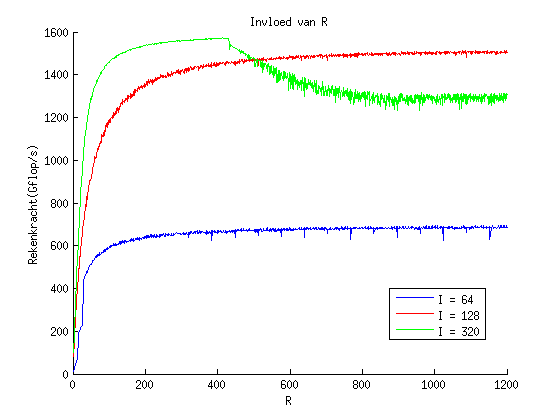
\includegraphics{invlR1200}
\caption{\label{invlR1200}Rekenkracht float16x16x16 voor verschillende waarden voor $R$ en $I$.}
\end{figure}

\begin{figure}
\centering
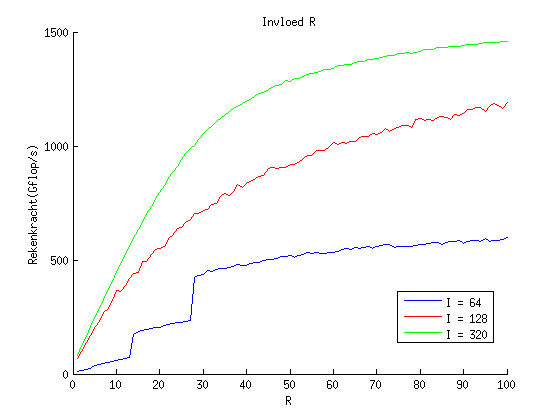
\includegraphics{invlR100}
\caption{\label{invlR100}Rekenkracht float16x16x16 voor verschillende waarden voor $R$ en $I$ met enkel de lage waardes van $R$.}
\end{figure}

\section{Invloed van I op kernels die $f(\T, \mUUU)$ berekenen}
\begin{figure}[h]
\centering
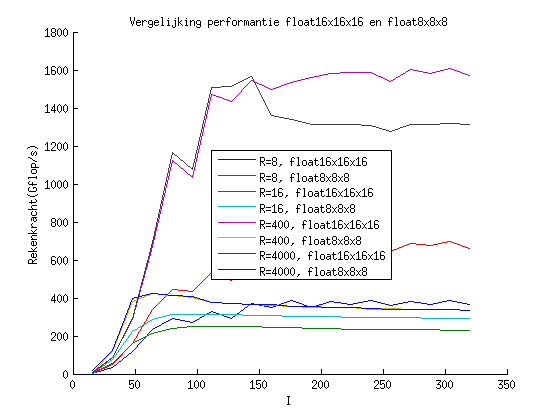
\includegraphics{fl16_vs_fl8_groot}
\caption{\label{fl16_vs_fl8} Vergelijking van de performantie tussen float16x16x16 en float8x8x8 voor verschillende waardes van $R$ en $I$.}
\end{figure}

We gebruiken in deze bespreking de kernels float16x16x16 en float8x8x8.
Voor elke kernel laten we $I$ oplopen van 16 tot en met 320 voor $R$ gelijk aan 8, 16, 400 en 4000. Zie figuur \ref{fl16_vs_fl8} voor de performantie van de kernels.

We laten $I$ oplopen in stappen van 16 omdat voor float16x16x16 $I$ een veelvoud moet zijn van 16. We beperken $I$ tot 320 omdat een buffer niet groter kan zijn dan 128MiB op onze grafische kaart. Als $I = 336$ dan moet de buffer om \TT{} op te slaan $336^3$ elementen $\times$ 4 B/element = 145MiB groot zijn.

We hebben voor $R$ de waardes 8 en 16 gekozen omdat dit twee punten zijn in de groeifase (zie figuur \ref{invlR100} en \ref{h:invlR}). $R=400$ is gekozen omdat het in de constante fase zit vlak voor dat rekenkracht terug naar beneden zakt. $R=4000$ is gekozen omdat het een hele grote waarde is die veel gewicht geeft aan de R-lus en dus heel performant moet zijn.

Bij $I$ = 16, 32 en 48 zien we een zeer sterke stijging van de performantie wanneer $I$ toeneemt. We kunnen die als volgt verklaren voor float16x16x16. Wanneer $I$ gelijk is aan 16 gebruiken we maar \'e\'en compute unit van de 24, wanneer $I$ gelijk is aan 32 gebruiken we er acht en bij 48 gebruiken we ze pas allemaal. Bij float8x8x8 gebruiken we voor $I=16$ acht CU's en vanaf $I=32$ alle CU's.

Nadat alle CU's in gebruik zijn zien we dat de rekenkracht nog steeds blijft stijgen. Dit komt omdat de CU's stil liggen wanneer alle work-groups op gegevens uit het globaal geheugen wacht. Door nog meer work-groups toe te wijzen aan een CU kunnen de CU's toch nog nuttige berekeningen doen terwijl andere work-groups op gegevens wachten. Dit verklaart waarom de rekenkracht toch sterk blijft stijgen nadat elke CU al minstens \'e\'en work-group uitvoert. Het is dus belangrijk om veel work-groups te voorzien.

Wanneer er genoeg work-groups zijn blijft de performantie min of meer constant. Bij float8x8x8 zien we amper schommelingen, terwijl we wel duidelijke schommelingen vaststellen bij float16x16x16. Merk wel op dat bij float16x16x16 de schommelingen gelijk lopen bij alle waardes van $R$.

Bij float16x16x16 met een $R=4000$ zien we dat bij $I=144$ de rekenkracht afneemt van 1566 Gflop/s naar ongeveer 1310 Gflop/s, net als bij \ref{h:invlR}. De verklaring is dezelfde als bij \ref{h:invlR}. Namelijk dat de caches niet zo goed meer werken.

Voor float16x16x16 zien we ook duidelijk dat de rekenkracht bijna lineair groeit met $R$ wanneer $R$ gelijk is aan 8 en 16. Wanneer $I$ groter is dan 150 is de rekenkracht bij $R=16$ bijna twee maal zo groot als bij $R=8$. Bij float8x8x8 is dat effect niet zo goed zichtbaar en is ook het verschil tussen $R=16$ en $R=400$ niet zo groot. Merk ook op dat bij float8x8x8 $R=400$ en $R=4000$ zo goed als volledig samenvallen.






\section{Vergelijking verschillende kernels die $f(\T, \mUUU)$ berekenen}
We hebben verschillende kernels ontwikkeld en willen die graag met elkaar vergelijken. Figuren \ref{fl16R_vs_fl16I}, \ref{fl16_vs_fl16R}, \ref{fl8_vs_fl8R} en \ref{fl16_vs_fl8} tonen de performantie van verschillende combinaties van de ontwikkelde kernels.

\subsection{Vergelijking tussen float16x16x16 en float16x16x16R}
\begin{figure}[h!]
\centering
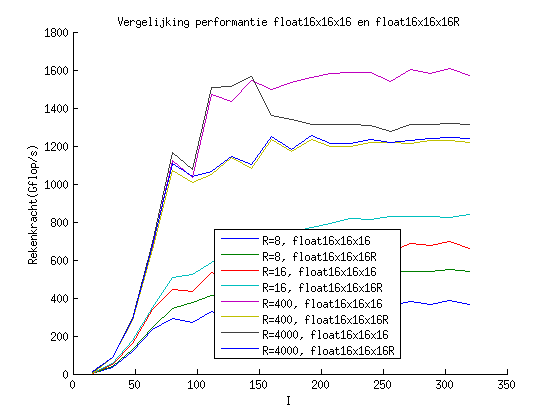
\includegraphics{fl16_vs_fl16R}
\caption{\label{fl16_vs_fl16R} Vergelijking van de performantie tussen float16x16x16 en float16x16x16R voor verschillende waardes van $R$ en $I$.}
\end{figure}

Float16x16x16R heeft als doel om het aantal geheugen conflicten te beperken. We willen graag zien of dit effectief gelukt is. Zie figuur \ref{fl16_vs_fl16R} voor een vergelijking van de performatie. We moeten een onderscheid maken tussen twee situaties. $R$ in de groeifase en $R$ in de constante fase.

Voor $R$ in de groeifase zien we dat float16x16x16R het duidelijk beter doet dan float16x16x16 wanneer $I$ wat groter is. Dit komt omdat in de groeifase de rekenkracht beperkt wordt door de bandbreedte. Door het aantal kanaalconflicten te verlagen kunnen we veel beter gebruik maken van die bandbreedte.

Wanneer $R$ in de constante fase is zijn de rollen omgekeerd. Na $I=96$ blijft de performantie van float16x16x16 verder groeien terwijl de performantie van float16x16x16R niet meer groeit.

Wanneer $I$ klein is zien we in alle gevallen dat float16x16x16 en float16x16x16R nagenoeg samenvallen. Dit komt omdat de kanaalconflicten dan nog niet het knelpunt is en dus slechts een beperkte, maar wel zichtbare, invloed hebben op de performantie.



\subsection{Vergelijking tussen float16x16x16R en float16x16x16I}
\begin{figure}[h!]
\centering
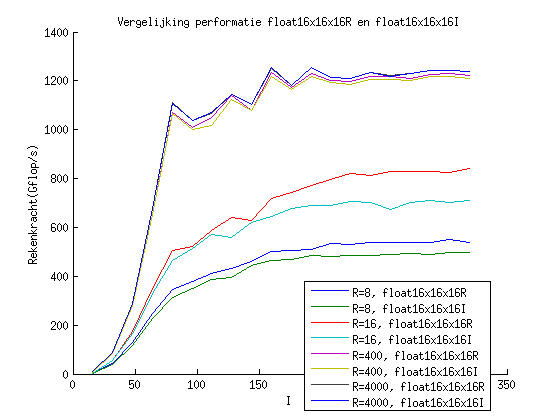
\includegraphics{fl16R_vs_fl16I}
\caption{\label{fl16R_vs_fl16I} Vergelijking van de performantie tussen float16x16x16R en float16x16x16I voor verschillende waardes van $R$ en $I$.}
\end{figure}

Float16x16x16R en float16x16x16I zijn beiden kernels die als doel hebben om het aantal geheugen conflicten te beperken. Zie figuur \ref{fl16R_vs_fl16I} voor een vergelijking van de performatie. We zien duidelijk dat float16x16x16R het overal beter doet dan float16x16x16I. Daarom gaan we verder geen aandacht meer besteden aan float16x16x16I.

\subsection{Vergelijking tussen float16x16x16 en float8x8x8}

\begin{figure}[h!]
\centering
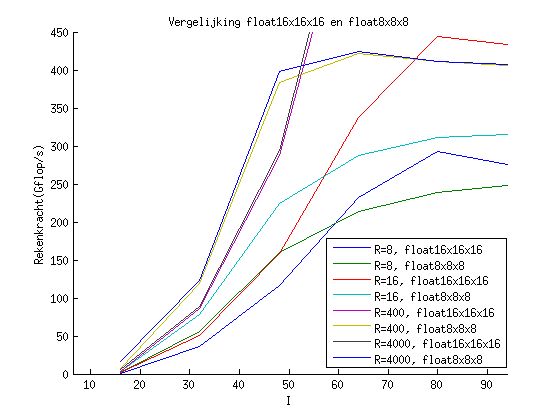
\includegraphics{fl16_vs_fl8_klein}
\caption{\label{fl16_vs_fl8_klein} Vergelijking van de performantie tussen float16x16x16 en float8x8x8 voor verschillende waardes van $R$ en $I$, uitvergroting snijpunten.}
\end{figure}

Zie figuur \ref{fl16_vs_fl8} voor een vergelijking tussen float16x16x16 en float8x8x8. Voor $I$ groter dan 64 zien we dat float16x16x16 veel beter presteert dan float8x8x8. Dit komt omdat float16x16x16 veel minder redundante berekeningen en geheugenoperaties moet doen dan float8x8x8. (Zie \ref{h:fl8_rekenverhouding} onder het punt 'Rekenverhouding')

Maar float8x8x8 heeft ook een voordelen. Omdat een work-group maar 8$\times$8$\times$8 groot is, zijn er meer work-groups nodig voor dezelfde hoeveelheid elementen. Waardoor de CU's beter benut worden. Zie figuur \ref{fl16_vs_fl8_klein} voor een beter zicht hierop. We zien dat float8x8x8 beter presteert dan float16x16x16 wanneer $I$ nog klein is. Het is pas later dat float16x16x16 de bovenhand haalt.

\subsection{Vergelijking tussen float8x8x8 en float8x8x8R}

\begin{figure}[h!]
\centering
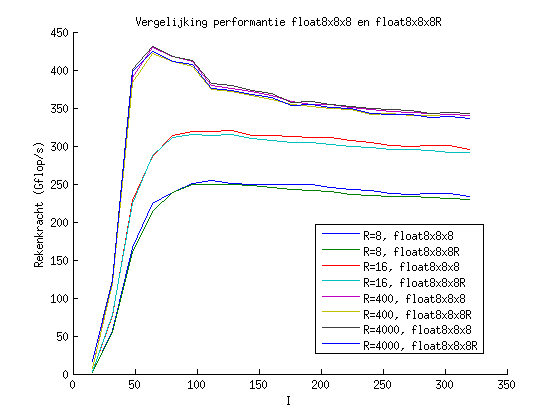
\includegraphics{fl8_vs_fl8R}
\caption{\label{fl8_vs_fl8R} Vergelijking van de performantie tussen float8x8x8 en float8x8x8R voor verschillende waardes van $R$ en $I$.}
\end{figure}

Zie figuur \ref{fl8_vs_fl8R} voor een vergelijking tussen float8x8x8 en float8x8x8R. We zien dat float8x8x8 het er overal een heel klein beetje beter doet dan float8x8x8R. We kunnen dus beter geen aandacht besteden aan float8x8x8R.

